\documentclass[a4paper,11pt]{article}
\usepackage[left=2.5cm, right=2.5cm, top=1.5cm, bottom=1.5cm]{geometry}
\usepackage{graphicx}
\usepackage{amssymb}
\usepackage{amsmath}
\usepackage{xcolor}
\usepackage[active,tightpage]{preview}
\usepackage{hyperref}
\usepackage{pythonhighlight}

\hypersetup{ %color attributes of citation, link, etc.
    colorlinks=true,
    linkcolor=blue,
    filecolor=gray,
    urlcolor=blue,
    citecolor=blue,
}

\setlength{\parindent}{0pt}

\renewcommand{\PreviewBorder}{1in}
\newcommand{\Newpage}{\end{preview}\begin{preview}}
\newcommand{\matlab}{\textsc{Matlab}} %very important and totally necessary addition
\newcommand{\parallelsum}{\mathbin{\!/\mkern-5mu/\!}}

\newcommand\Item[1][]{%
  \ifx\relax#1\relax  \item \else \item[#1] \fi
  \abovedisplayskip=0pt\abovedisplayshortskip=0pt~\vspace*{-\baselineskip}}

%'codify' text for snippets
\usepackage{xcolor}
\definecolor{codegray}{gray}{1}
\newcommand{\code}[1]{\colorbox{codegray}{\texttt{#1}}}


\graphicspath{ {../images/} }
           
\begin{document}
\begin{preview}
\title{\LARGE{\textbf{ECEN415 Assignment 1}}}
\author{Niels Clayton : 300437590}
\date{}
\maketitle
\hrule

\begin{enumerate}
    
    \item Sketch Nyquist plots

    \begin{enumerate}
      \item $$ G_1 (s) = \frac{20(s^2+s+0.5)}{s(s+1)(s+10)} $$
      
      \begin{center}
        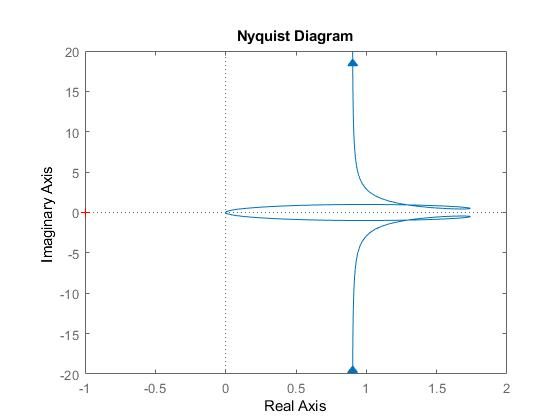
\includegraphics[width=0.7\textwidth]{A_1/1_a.jpg}
      \end{center}

      This system is stable initially, with no right hand poles in the open loop function, and no encirclements of the critical point. However negative gain will cause the closed loop system to become unstable.\\
      

      \item $$ G_2 (s) = \frac{20(s^2+s+0.5)}{s(s-1)(s+10)} $$

      \begin{center}
        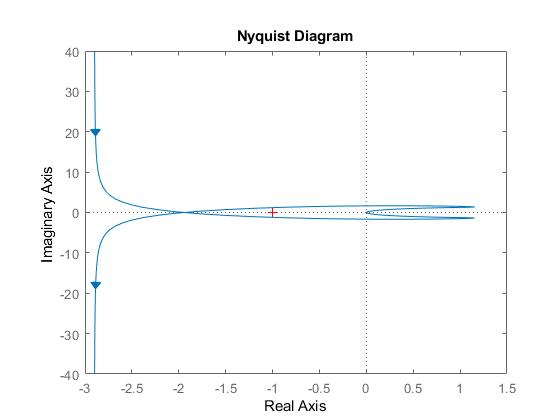
\includegraphics[width=0.7\textwidth]{A_1/1_b.jpg}
      \end{center}

      This system is stable initially, with one right hand poles in the open loop function, and single anticlockwise encirclement of the critical point. However negative gain will cause the closed loop system to become unstable.\\


      \item $$ G_3 (s) = \frac{ s^2+3 }{ (s+1)^2 } $$

      \begin{center}
        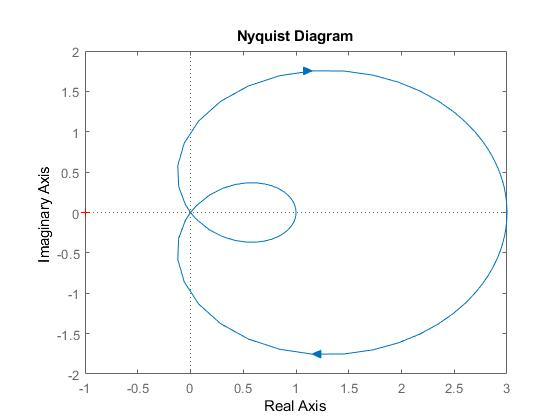
\includegraphics[width=0.7\textwidth]{A_1/1_c.jpg}
      \end{center}

      
      This system is stable initially, with no right hand poles in the open loop function, and no encirclement of the critical point. However negative gain will cause the closed loop system to become unstable, adding up to two anticlockwise encirclements depending on the negative gain.\\


      \item $$ G_4 (s) = \frac{ 3(s+1) }{ s(s-10) } $$

      \begin{center}
        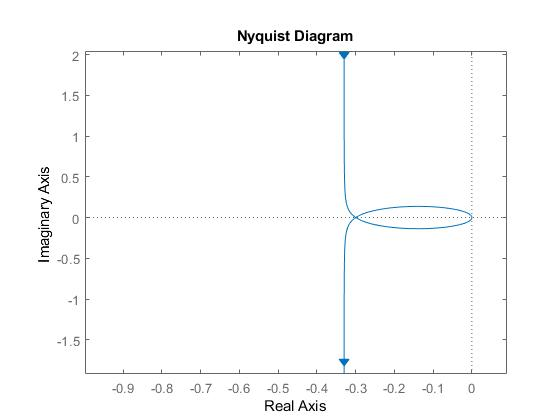
\includegraphics[width=0.7\textwidth]{A_1/1_d.jpg}
      \end{center}

      This system is unstable initially, with one right hand pole in the open loop function, and no encirclement of the critical point. However positive gain will cause the closed loop system to become stable, adding an anticlockwise encirclement of the critical point.\\
    \end{enumerate}


\hrule

\item 

\end{enumerate}

\end{preview}
\end{document}